\documentclass{article}

% if you need to pass options to natbib, use, e.g.:
% \PassOptionsToPackage{numbers, compress}{natbib}
% before loading nips_2018

% ready for submission
% \usepackage{nips_2018}

% to compile a preprint version, e.g., for submission to arXiv, add
% add the [preprint] option:
% \usepackage[preprint]{nips_2018}

% to compile a camera-ready version, add the [final] option, e.g.:
\usepackage[final]{nips_2018}

% to avoid loading the natbib package, add option nonatbib:
% \usepackage[nonatbib]{nips_2018}

\usepackage[utf8]{inputenc} % allow utf-8 input
\usepackage[T1]{fontenc}    % use 8-bit T1 fonts
\usepackage{hyperref}       % hyperlinks
\usepackage{url}            % simple URL typesetting
\usepackage{booktabs}       % professional-quality tables
\usepackage{amsfonts}       % blackboard math symbols
\usepackage{nicefrac}       % compact symbols for 1/2, etc.
\usepackage{microtype}      % microtypography
\usepackage{graphicx}
\usepackage{mathtools}
\usepackage{amsmath}
\usepackage{bbm}
\title{Deep Learning 2018 - Assignment 2}

% The \author macro works with any number of authors. There are two
% commands used to separate the names and addresses of multiple
% authors: \And and \AND.
%
% Using \And between authors leaves it to LaTeX to determine where to
% break the lines. Using \AND forces a line break at that point. So,
% if LaTeX puts 3 of 4 authors names on the first line, and the last
% on the second line, try using \AND instead of \And before the third
% author name.

\author{
  David Rau (11725184) \\ 
  University of Amsterdam \\
  \texttt{david.rau@student.uva.nl} \\
  %% examples of more authors
  %% \And
  %% Coauthor \\
  %% Affiliation \\
  %% Address \\
  %% \texttt{email} \\
  %% \AND
  %% Coauthor \\
  %% Affiliation \\
  %% Address \\
  %% \texttt{email} \\
  %% \And
  %% Coauthor \\
  %% Affiliation \\
  %% Address \\
  %% \texttt{email} \\
  %% \And
  %% Coauthor \\
  %% Affiliation \\
  %% Address \\
  %% \texttt{email} \\
}

\begin{document}
% \nipsfinalcopy is no longer used

\maketitle


\section*{Vanilla RNN versus LSTM}
\subsection*{Vanilla RNN in PyTorch}
\subsubsection*{Question 1.1}
\begin{equation}
\begin{aligned}
	\frac{\partial L^{(T)}}{\partial W_{ph}} & = \frac{\partial L^{(T)}}{\partial \hat{y}^{(T)}}\frac{\partial \hat{y}^{(T)}}{\partial p^{(T)}}\frac{\partial p^{(T)}}{\partial W_{ph}} \\
	&= \frac{\partial \Big(-\sum_{k=1}^K y_k \log \hat{y}_k \Big)}{\partial \hat{y}^{(T)}} \frac{Softmax(p^{(T)})}{\partial p^{(T)}}\frac{\partial \Big(W_{ph} h^{(T)} + b_p \Big)}{\partial W_{ph}} \\
	& = -\frac{1}{\hat{y_i}}\mathbbm{1}(i=\operatorname{argmax}_t )  Softmax(\hat{y_i})(\delta_{i,j}-Softmax(\hat{y_j})) h^{(T)}
\end{aligned}
\end{equation}



\begin{equation}
\begin{aligned}
	\frac{\partial L^{(T)}}{\partial W_{hh}} & = \sum_{k=0}^T \frac{\partial L^{(T)}}{\partial \hat{y}^{(T)}}\frac{\partial \hat{y}^{(T)}}{\partial p^{(T)}}\frac{\partial p^{(T)}}{\partial h^{(T)}} \prod_{j=k+1}^{T} \frac{\partial h^{(j)}}{\partial h^{(j-1)}} \frac{\partial h^{(k)}}{\partial W_{hh}}\\
	& = \sum_{k=0}^T  \frac{\partial \Big(-\sum_{k=1}^K y_k \log \hat{y}_k \Big)}{\partial \hat{y}^{(T)}} \frac{Softmax(p^{(T)})}{\partial p^{(T)}}\frac{\partial \Big(W_{ph} h^{(T)} + b_p\big)}{\partial h^{(T)}} \prod_{j=k+1}^{T} \frac{\partial \Big(tanh(W_{hx}x^{(j)} + W_{hh} h^{(j-1)} + b_h) \Big)}{\partial h^{(j-1)}} \\
	& \frac{\partial \Big(tanh(W_{hx}x^{(k)} + W_{hh} h^{(k-1)} + b_h) \Big)}{\partial W_{hh}} \\
	& =\sum_{k=0}^T  -\frac{1}{\hat{y_i}}\mathbbm{1}(i=\operatorname{argmax}_t )  Softmax(\hat{y_i})(\delta_{i,j}-Softmax(\hat{y_j})) h^{(T)} \prod_{j=k+1}^{T} \big( 1-h^{(j)2} \big)  W_{hh} \big( 1- h^{(k)2} \big) h^{(k-1)} 
\end{aligned}
\end{equation}


\subsubsection*{Question 1.3}
The plot that shows the accuracy versus palindrome length of the Vanilla RNN can be found in the answer of Question 1.6.
\subsubsection*{Question 1.4}
Vanilla Stochastic Gradient Decent yields a gradient in direction of the steepest decent. However, following the steepest decent might not lead to an optimal local minimum. SGD converges to the closest minimum in the loss surface if the direction of the steepest decent points towards it, even though there is a better minimum very close by. This can be overcome by making use of the \textbf{momentum term}. Momentum is inspired by the physical laws of motion. An object gains momentum while moving downhill and is able to overcome small hills on its way to the lowest point on the surface where it eventually stops. Similarly, adding a momentum term  that takes into account the direction of the gradients from previous time steps the gradient becomes more stable (also against oscillation) and is potentially able surpass suboptimal local minima. \\
Another technique to avoid being stuck in local minima is to \textbf{change the learning rate over time}. Is the learning rate to small it takes too long to converge to a good optimum, is it so big a good optimum could be skipped. The solution to this is starting with a big learning rate and then decreasing the learning in chosen intervals. 
\subsection*{Long-Short Term Network (LSTM) in PyTorch}
\subsubsection*{Question 1.5 (a)}
\textbf{input modulation gate g:}  This gate updates the cell state through two components: the previous cell state multiplied with the forget gate and the input that the input gate decided to let into the network. Tanh is used to obtain the non-linearity and to scale the output to [-1,1]. This can also stabilise the gradients throughout the recurrency.  \\

\textbf{input gate i:} To regulate the information inflow into the cell. The idea is to either let all information flow into the cell or none. Like a switch. To modulate this a sigmoid function is used. \\

\textbf{forget gate f:} To be able to no indefinitely accumulate information over time, but be able to reset the cell state. Sigmoid is used because of the same reason as for i. \\

\textbf{output gate o:} To regulate the information outflow into the cell. Sigmoid is used because of the same reason as for i. \\
\subsubsection*{Question 1.5 (b)}
\begin{equation}
	4(d \times n + n^2 + n)
\end{equation}
I only took into account the core equations of a LSTM cell (eq. 4-9 on the assignment sheet).
\subsubsection*{Question 1.6}
For this exercise the long range dependencies of a simple Vanilla RNN and an LSTM models are probed.  We train on the Palindrome task that is to predict the last character of a symmetric sequence of characters.
The plot that shows the maximal batch accuracy during the whole training procedure plotted against the sequence length of both models can be found in Fig. \ref{rnn_lstm_comparison}. Each of the models was trained with the default parameters (learning rate: 0.001, batch size: 128, hidden units: 128, max. steps: 10000) initially. As it can be seen in Fig. \ref{rnn_lstm_comparison} the LSTM with the default learning rate outperforms the Vanilla RNN but the performance collapses from 100\% to around 30\% for sequence length 20. Knowing that LSTMs are, at least in theory, able to keep long distance relationships indefinitely long and that the gradient vanishes with an increasing sequence length, increasing the learning rate should boost the performance. The results show that the LSTM with learning rate 0.01 yields a perfect performance (accuracy 100\%) for all sequence lengths, whereas the Vanilla RNN fails to predict the last character (accuracy $<$ 30\%) from length 11 on.
\begin{figure*}[h!]
    \centering
  \centering
  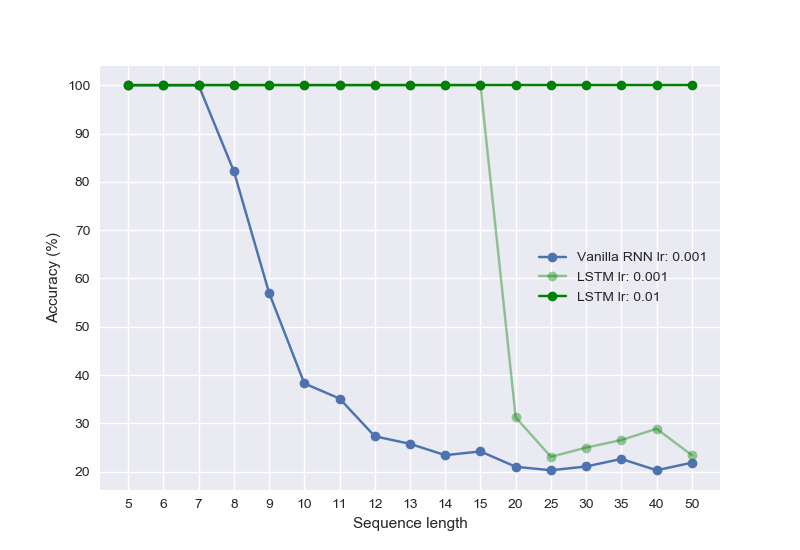
\includegraphics[scale=0.45]{Figure_1}
  \caption{Highest batch accuracy (\%) during the training of the Vanilla RNN (blue) and LSTM (green) plotted against different Sequence lengths. The LSTM model was trained with two different learning rates 0.01 and 0.001. }
  \label{rnn_lstm_comparison}
\end{figure*}
\newpage
\section*{Modified LSTM Cell}
\subsubsection*{Question 2.1}
\begin{figure*}[h!]
    \centering
  \centering
  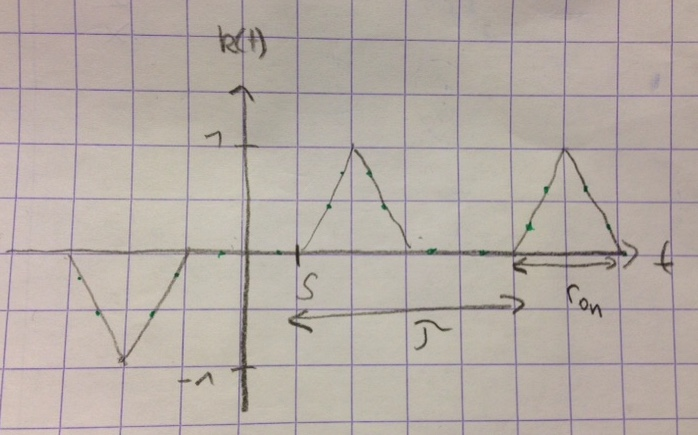
\includegraphics[scale=0.3]{sketch}
  \caption{Conceptual drawing of the change of gate $k^{(t)}$ over time $t$.}
\end{figure*}
\subsubsection*{Question 2.2}
When the gate $k^{(t)}$ is close to 1 the new cell $c^{(t)$ and hidden state $h^{(t)$ are mostly dependent on the current candidate cell and hidden states $\tilde{c}^{(t)$ and $\tilde{h}^{(t)$ respectively. If $k^{(t)}$ is close to 0 the new cell $c^{(t)$ and hidden state $h^{(t)$ are mostly dependent on the previous cell $c^{(t-1)$ and hidden state $h^{(t-1)$ respectively. This behaviour could be beneficial in cases where periodic processes are to be modelled where the update of the cell and hidden state depends on the ratio of the previous and the current state and is conditioned on the time. In this case the memory cell is rarely updated and most of the times the cell and hidden state solely dependent on the candidate states. 
\subsubsection*{Question 2.3}
s is responsible for the phase shift. $\tau$ is responsible for the periodicity of the updates of the memory cell. $r_{on}$ is responsible for the duration that the memory cell is updated. All parameters can be learned.

\newpage
\subsubsection*{Question 3.1 (b)}
Examples: \\

\textbf{Epoch 1 Step 200:}\\
n der der der der der der der 	\\nder der der der der der der d \\	er der der der der der der der\\	en der der der der der der der\\	en der der der der der der der\\

\textbf{Epoch 4 Step 200:}\\ en der Hungerkuenstler vor die	\\enen war das ein allei er nich \\	r sie er die Staren das Hunger\\	mpresario ein Tier an dem Grue\\	eit gescheinen war das Hungern\\

\textbf{Epoch 7 Step 200:}\\ r der Hungerkuenstler selbst k	\\ Wer es nicht aufhaechst einma \\	r den Hungerkuenstler vor dies\\	echtig vortretenden Rippen, so\\	ielleicht war er gar nicht an\\

\textbf{Epoch 10 Step 200:}\\  der Hungerkuenstler selbst ko	\\rer waren ihm die Waechter, we \\	uem ansehen wollte, nicht etwa\\	 sich hier handelte, von frueh\\	 sich hier handelte, von frueh\\

In epoch 1 we can see that the model has only picked up the very common word 'der' an repeats it. From epoch 4 on the model is able to generate sentences that resemble those of the book that it was trained on. Words are capitalised and the grammar resembles the german language. Because greedy sampling is used the generated words are repetitive and are mostly made up from the most frequent words in the corpus. This makes the word generation from a time point on deterministic. From epoch four on there is no difference between the forthcoming epochs is observable. The fast convergence could be due to the relatively small book that was chosen. 

\subsubsection*{Question 3.1 (c)}
Examples: \\

\textbf{temp: 0.5} \\
uschauer sein, sondern aus Lau	\\
er der sich heranwaelzenden M	\\
er zu bewahren, dann aber vers	\\
ch, immer wieder zeigen zu koe	\\
ar das Hungern war. Es war die	\\


\textbf{temp: 1} \\
er Glueckssalt, dass vererwarl	\\
hies zu hungern, warum wollte	\\
orangewaehrend es ein feurigen	 \\
weiler im Eich herorommertr? 	\\
ch hatte sich im Seinen seisen\\

\textbf{temp: 2} \\
Schwung eingetreten; fast plo	\\
Lanpfem guense Gndeit. fote. 	\\
lhu Et? sein gech ansehingeluc\\
austler darin. Du hungerspaech	\\
hmung. De niemals gwuesschmet.\\

With an increasing number of the temperature it can be noted that the sentences become more versatile and and challenge the model to use words that are less frequent in the training corpus. On the other hand by not using the character with the highest probability of the model the words contain a lot of spelling mistakes. By using temperature 1 the sentences still resemble german but are not understandable. Temperature 2 generates fantasy words with an german origin. 


\subsubsection{Bonus Question 3.3}

Example generated with length  200:

 seine Kberig aubhiede enden Hungertag zu Hungertag stieg die Teilnahme; jeder wollte den Hungerkuenstler zu bewahren, dann aber versagte das Publikum, eine wesentliche Vorbeterte de das Stroh aruene
 
\end{document}
